% Working preprint. The template's preprint option makes no review-status claim.
\documentclass[10pt]{article}
\usepackage[preprint]{tmlr-style/tmlr}
\usepackage{amsmath,amssymb,amsthm,booktabs,graphicx,hyperref}
\hypersetup{hidelinks}
\newtheorem{theorem}{Theorem}
\newtheorem{proposition}{Proposition}
\newtheorem{corollary}{Corollary}
\newtheorem{lemma}{Lemma}
\newcommand{\ind}{\mathbf{1}}
\emergencystretch=2em
\title{When Threshold Sampling Reverses VUS Rankings:\\
Exact and Certified Evaluation of Anomaly Scores}
\author{\name Youngmin Ko \email rhdudals0505@naver.com\\
\addr Independent Researcher, Republic of Korea}
\begin{document}
\maketitle
\begin{abstract}
Volume Under the Surface (VUS) compares anomaly scores across temporal
tolerance widths and score thresholds.\footnote{LLM assistance was used in
literature search, mathematical derivation, implementation, experiment
orchestration, and drafting. Verification used independent implementations,
exact rational checks, pinned upstream controls, and frozen evidence;
agent reviews were internal checks, not external peer review.}
Its mathematical definition can
be threshold-independent while a finite integration grid remains
inaccurate. We analyze a specific failure of the original dynamic VUS-PR:
soft-label mass admitted after exhaustive recall saturates can inflate
the precision assigned to an earlier recall jump. We give a finite
worst-case overestimation bound exceeding 0.98 and same-label, distinct-score
constructions at 250 thresholds with exact-score selection regret of
0.507, 0.701 and 0.846 at maximum widths 30, 100 and 300.
We derive bidirectional error enclosures and implement them with integer
square roots and directed integer arithmetic, certifying the ideal
real-arithmetic target without relying on a floating-point tolerance.
A prospectively selected panel re-evaluates 1,536 published detector score
vectors on 128 time series from sixteen source families. At width 30,
the default grid selects a model with exhaustive regret at least 0.01
on eight series across four families; the largest regret is 0.399.
Integer enclosures prove all eight regret claims and the unique
exhaustive winner on all 128 series. Partial grids certify 63 winners
at 250 thresholds and 94 at 1,000. All stored score vectors have at most
101 distinct values: requesting more ranks than distinct scores does
not ensure exhaustive integration. We report source-overlap sensitivity,
signed errors, matched exhaustive controls, and certification costs.
\end{abstract}

\section{Introduction}
An anomaly detector produces scores; an evaluation procedure turns those
scores into evidence for comparing or selecting models. Approximation in
the evaluator can therefore affect the scientific conclusion even when
the labels, models, and score vectors do not change. Volume Under the
Surface (VUS) extends range-aware ROC and PR areas by averaging across
temporal tolerance widths~\citep{paparrizos2022,boniol2025}. This work
studies fidelity to one explicitly pinned VUS-PR definition, rather than
whether that metric is the best proxy for a deployment's utility.

Finite-threshold approximation is well known. Classical work shows that
PR interpolation differs from ROC interpolation~\citep{davis2006}, and
weighted PR requires additional care~\citep{keilwagen2014}. Keras documents
finite-threshold errors and bounding estimates~\citep{kerasauc}; TimeEval
also warns about coarse VUS threshold grids~\citep{timeevalvus}.
PAULA derives sampled-rank precision bounds under explicit monotonicity
assumptions in an annotation-budget setting~\citep{sabharwal2017}. Generic
claims that approximation loses information, or that evaluation metrics
can change a ranking, would add little to this literature.

Our specific observation concerns a dynamic soft-label target in which
recall is clipped before all soft positive mass has entered. Precision can
continue increasing after recall reaches one. A sampled threshold can
assign this later precision to a recall jump that happened at a much
lower precision. The corresponding exhaustive integral assigns zero area
to the post-saturation mass. This produces a qualitatively different
mechanism from the familiar loss of early positive ranks under coarse
sampling. Figure~\ref{fig:mechanism} illustrates the mechanism and large
same-label ranking reversals at ordinary maximum widths.

\begin{figure}[t]
\centering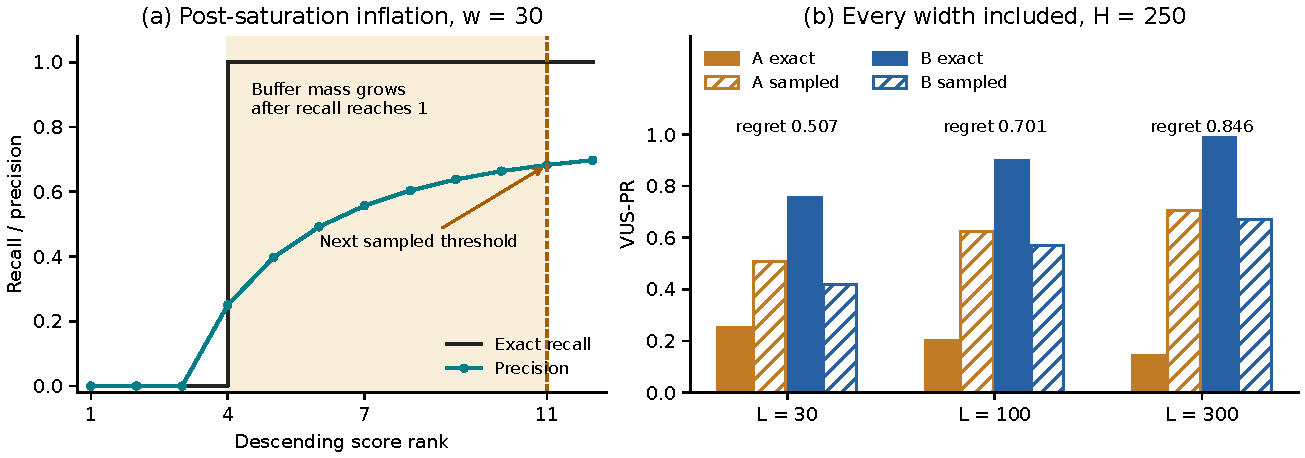
\includegraphics[width=\linewidth]{figures/sampling_witnesses.pdf}
\caption{Constructed failures, not prevalence estimates. Left: after the
sole original positive enters at rank four, recall is one while buffer
mass keeps increasing precision. The next retained threshold is rank
eleven. Right: all-width averages at the standard 250-threshold budget
prefer score vector A although exhaustive evaluation prefers B.}
\label{fig:mechanism}
\end{figure}

We provide three forms of evidence. First, explicit constructions and
proofs establish what the approximation can do, including large finite
overestimation and selection regret. Second, a mass-envelope analysis
yields intervals that can certify the exhaustive ordering of models, with
an integer implementation that preserves the mathematical guarantee.
Third, a fixed, previously unmeasured bank of twelve released score
configurations per series separates worst-case possibility from observed
effects and computational costs. The score bank is used for offline
evaluation with labels, not label-free selection at deployment.

A publicly released support-event evaluator supplies the numerical
exhaustive baseline~\citep{sparsevus03}. We do not relabel that earlier
implementation, its already measured speedups, ordinary radix sorting, or
generic PR error bounds as new discoveries. The new investigation isolates
post-saturation inflation, a sound integer remedy, and its consequences on
a broader published detector panel. Likewise, certification of a ranking
does not certify the detector's real-world usefulness.

\section{Sampling can inflate the dynamic PR integral}
\label{sec:sampling-inflation}
Fix the original dynamic VUS-PR contract for $n$ binary labels with both
classes present, $0<P_0<n$, finite scores, and a nonnegative integer
maximum width $L$. The implementation evaluates the scores after its
documented binary64 conversion. At width $w$, original positives
have unit weight and each interval adds a square-root ramp
$\sqrt{1-d/w}$ at distances $1\leq d\leq\lfloor w/2\rfloor$;
overlapping contributions are summed and clipped at one. At a complete
score threshold, let $C$ be the predicted count, $A$ the admitted original
positive count, $B$ the admitted buffer mass, $P_0$ the total original
positive count, and $h/K_w$ the fraction of expanded components hit.
Overlapping expanded intervals merge, whereas adjacent nonoverlapping
intervals remain distinct. The coordinates are
\[
 T=A+B,\qquad P=P_0+B/2,\qquad
 R=\min(T/P,1)h/K_w,\qquad \pi=T/C.
\]
The exhaustive PR area is $\sum_j(R_j-R_{j-1})\pi_j$, beginning at
$R_0=0$ and admitting each distinct global score tie completely. VUS-PR
averages this area over every integer width $0,\ldots,L$.

The sampled implementation retains descending zero-based ranks
\texttt{linspace(0,n-1,H).astype(int)}, with $H=250$ by default
in both the official VUS optimized API~\citep{officialvuscode} and
the pinned fast-VUS source~\citep{klein2026}. It uses the same PR
integral on those retained states. Sampling error is different from a
change of metric semantics or an implementation defect: the upstream
routine correctly computes its configured sampled target.

The important feature is that precision can increase \emph{after} recall
has already reached one. Additional buffer mass then contributes zero
exhaustive area, but a coarse threshold can incorrectly assign that later
precision to a recall jump which occurred earlier. Binary average
precision cannot add positive mass after every original positive has
already been admitted. The following construction isolates the additional
soft-label mechanism.

\begin{proposition}[A parameterized sampling family]
\label{prop:overshoot-family}
Let $H\geq2$, $1\leq m<q$, $n=1+(H-1)q$, and
$\lfloor L/2\rfloor<n-m$. Put a single original positive at temporal
position zero. Assign distinct descending scores first to the last $m$
positions, then to position zero, and then to positions
$1,\ldots,n-m-1$ in temporal order. The exhaustive VUS-PR equals
$E=1/(m+1)$, whereas its $H$-threshold sampled value is
\begin{equation}
 S=\frac{1+(L+1)^{-1}\sum_{w=0}^L B_w}{q+1},\qquad
 B_w=\sum_{d=1}^{\min(q-m,\lfloor w/2\rfloor)}\sqrt{1-d/w},
 \label{eq:overshoot-value}
\end{equation}
where the empty sum at $w=0$ is zero. The sign of $S-E$ depends on the
parameters; the overestimation regimes below are separate conclusions.
\end{proposition}
\begin{proof}
The first $m$ positions are outside every evaluated support. At actual
rank $m+1$, admitting the sole original positive makes both coverage and
clipped recall one. The entire exhaustive recall increase therefore has
precision $1/(m+1)$, independently of width. Later recall increments vanish.
The retained one-based ranks are exactly $1,1+q,\ldots,n$. Recall at the
first is zero; recall at the second is one, and the second includes the
original plus the nearest $q-m$ positions. Its precision is
$(1+B_w)/(q+1)$, proving the formula after averaging widths.
\end{proof}

\begin{corollary}[Large finite overestimation]
\label{cor:large-overshoot}
For $H=250$ there is a finite member of
Proposition~\ref{prop:overshoot-family} with $S-E>0.98$.
\end{corollary}
\begin{proof}
For $L\geq2q$, retain only widths $2q,\ldots,L$ and use
$\sqrt{1-x}\geq1-x$ to obtain
\[
 S\geq\frac{(L-2q+1)(q-m+1)
       -\frac{(q-m)(q-m+1)}2\sum_{w=2q}^Lw^{-1}}
       {(L+1)(q+1)}.
\]
Take $q=2{,}000{,}000$, $m=1000$, $n=498{,}000{,}001$ and
$L=498{,}000{,}000$. The harmonic tail is less than
$\log(L/(2q-1))<5$; the latter inequality follows, for example, from
the degree-seven positive Taylor lower bound for $\exp(5)$.
Thus $S>977516488501501/996000500000001$. Exact rational subtraction
of $E=1/1001$ exceeds $98/100$.
\end{proof}
This finite statement was verified symbolically, without allocating the
large input or executing an evaluator on it. Its maximum width is $n-1$;
it is not a claim about a typical small tolerance width. More generally,
with fixed $H>3$, $L=(H-1)q$, $m\to\infty$ and $m/q\to0$,
\[
 \liminf S\geq1-\frac2{H-1}
                   -\frac{\log((H-1)/2)}{2(H-1)},\qquad E\to0.
\]
This asymptotic family is a real-arithmetic statement, rather than an
unbounded supply of distinct binary64 scores.

\paragraph{Large selection regret at ordinary fixed widths.}
For a second score vector on the same labels, place a nearby buffer
position $d$ first and the original second. Fill the remaining $q-1$
positions through rank $q+1$ with far outside-support negatives; rank
everything else later. Sufficient feasibility conditions are
$n-q+1>\lfloor L/2\rfloor$ and $1\leq d<n-q+1$.
At $w<2d$ the exhaustive and sampled areas are respectively
$1/2$ and $1/(q+1)$. Otherwise, writing
$a=\sqrt{1-d/w}$ and $r=a/(1+a/2)$ gives
\[
 E_B(w)=ra+(1-r)(1+a)/2,\quad
 S_B(w)=ra+(1-r)(1+a)/(q+1).
\]
Table~\ref{tab:constructed-reversal} reports complete width averages.
All scores are distinct finite integers. Closed forms, independent dense
evaluation, compiled exhaustive evaluation, and unchanged pinned upstream
calls at $H=250$ and $H=n$ agree numerically. These are exploratory
constructed witnesses of possibility, not estimates of prevalence.

\begin{table}[t]
\centering\small
\begin{tabular}{rrrrrrrr}
\toprule
$L$ & $n$ & $(q,m,d)$ & $E_A$ & $S_A$ & $E_B$ & $S_B$ & regret\\
\midrule
30 & 2491 & $(10,3,5)$ & .250000 & .506412 & .757142 & .418181 & .507142\\
100 & 4981 & $(20,4,5)$ & .200000 & .624743 & .900580 & .569008 & .700580\\
300 & 9961 & $(40,6,1)$ & .142857 & .706289 & .989249 & .668767 & .846392\\
\bottomrule
\end{tabular}
\caption{Same-label reversals with $H=250$. Sampling selects A; exhaustive
evaluation selects B. Regret is $E_B-E_A$, measured in exhaustive VUS-PR
units and not in an operational detection utility.}
\label{tab:constructed-reversal}
\end{table}

\section{Sound bounds from retained threshold states}
\label{sec:threshold-certificate}
An approximation can be accompanied by a checkable interval instead of
being treated as an exact scalar. The general idea of bounding numerical
quadrature is established; our result supplies a bound for this dynamic,
clipped-recall, soft-label target without assuming monotone precision.

\begin{theorem}[Mass-envelope PR enclosure]
\label{thm:threshold-enclosure}
At one width, consider two consecutive retained complete-threshold states
$(c_a,t_a,r_a)$ and $(c_b,t_b,r_b)$, including an initial zero state and
discarding repeated states. Put $\delta=t_b-t_a$ and
\[
 \ell=\frac{t_a}{c_b-\delta},\qquad
 u=\frac{t_b}{c_a+\delta}.
\]
If $c_b-\delta=0$, set $\ell=1$; a zero-mass block contributes zero.
The exhaustive PR area inside this block is between
\begin{equation}
 \int_{r_a}^{r_b}\max(\ell,P_0r/c_b)\,dr
 \quad\text{and}\quad (r_b-r_a)u.
 \label{eq:block-bounds}
\end{equation}
Summing these bounds over blocks and averaging widths encloses exhaustive
VUS-PR. In particular, disjoint model intervals certify their exact order.
\end{theorem}
\begin{proof}
Every temporal weight lies in $[0,1]$. At an intermediate predicted count
$c$, its true mass $t$ satisfies
\[
 \max(t_a,t_b-c_b+c)\leq t\leq\min(t_b,t_a+c-c_a).
\]
Dividing by $c$ and optimizing the two continuous piecewise envelopes
gives $\ell\leq t/c\leq u$. Optimizing over continuous counts is safe
for integer counts and complete ties because it enlarges the feasible
set. If the lower denominator vanishes, all admitted weights are one.

Recall is nondecreasing along descending scores: $(A+B)/(P_0+B/2)$
increases in $A$ and $B$, with derivative in $B$ proportional to
$P_0-A/2>0$. Clipping and multiplication by nonnegative, nondecreasing
coverage preserve this property. Thus all recall increments are nonnegative.
Also $T\geq P_0R$, and $C\leq c_b$, so contributing precision is at
least $P_0R/c_b$. The exact right-step sum dominates the integral of the
nondecreasing lower envelope; its upper bound follows by summing recall
increments times $u$.
\end{proof}

The bound is elementary and can be loose. Refining a retained grid
monotonically tightens the real-arithmetic enclosure: $c-t$ is
nondecreasing, so each subblock has a lower mass envelope at least as
large, an upper envelope no larger, and a no-smaller linear lower envelope.
If consecutive global distinct-score ordinals establish that no valid
threshold was omitted, use the observed exact right-step term instead.
A complete tie can admit many positions without containing any valid
intermediate threshold.

\paragraph{An information limit.}
Endpoint-only bounds cannot always be narrow. Fix $H\geq3$ and $L$;
choose one original interval of $m$ points and a sampling gap $q\gg m+L$.
Two score orders can put those originals immediately after the first
off-support negative, or at the end of the same gap, while giving identical
$(C,A,B,h)$ at every retained threshold and every width. Their exhaustive
areas are obtained by placing the entire maximum-width halo in a common
tail after that gap and filling the remaining gap with off-support points.
Recall saturates before the common halo enters. The exhaustive
areas are respectively
\[
 \frac1m\sum_{j=1}^m\frac{j}{j+1},\qquad
 \frac1m\sum_{j=1}^m\frac{j}{q+1-m+j}.
\]
The first tends to one and the second to zero as $m\to\infty$ and
$q/m\to\infty$. A bound valid for every score ordering consistent with
that retained transcript must include both. This is an ordinary ranking
information-loss argument; it does not lower-bound methods that inspect
omitted support scores or adapt their thresholds.

\section{Integer-directed realization}
\label{sec:integer-certificate}
Theorem~\ref{thm:threshold-enclosure} concerns real arithmetic. Adding a
floating-point tolerance to a numerical check would not implement that
guarantee. We instead construct dyadic enclosures using integer square
roots and directed integer division.

Let $D=2^{32}$ be the weight scale. For a single ramp at distance $d$,
set $z=(w-d)D^2$ and $q=\operatorname{isqrt}(\lfloor z/w\rfloor)$.
Then $q/D\leq\sqrt{1-d/w}\leq(q+1)/D$, with exact upper numerator
$q$ when $q^2w=z$. Original positives and points covered by two ramps have
exact numerator $D$; inactive points have zero. Since every active ramp
is at least $1/\sqrt2$, two ramps indeed clip to one. For $n<2^{31}$,
all compiled signed-64-bit cumulative buffer sums are below $2^{63}$.
Nonlinear calculations and final sums use arbitrary-precision Python
integers; public NumPy integer parameters are normalized before them.

For an endpoint with exact original count $A$, buffer brackets
$[B_-,B_+]/D$, and exact hit count $h$, use
\[
 f(B)=\frac{h\min\{2(AD+B),\,2P_0D+B\}}
              {K_w(2P_0D+B)}.
\]
Monotonicity gives $f(B_-)\leq R\leq f(B_+)$. With output scale
$S=2^{56}$, floor the lower product $Sf(B_-)$ and ceil the upper
product $Sf(B_+)$. Both endpoint precision envelopes can be rewritten
as functions nondecreasing in each total-mass argument:
\[
 \ell(t_a,t_b)=\frac{t_a}{c_b-t_b+t_a},\qquad
 u(t_a,t_b)=\frac{t_b}{c_a-t_a+t_b}.
\]
Substitute both lower mass endpoints into $\ell$ and both upper
endpoints into $u$. Combine these rational precision bounds with directed
recall differences. When $R_a^+<R_b^-$, the linear lower refinement is
integrated analytically over $[R_a^+,R_b^-]$, a subset of the actual recall
interval; otherwise that refinement contributes zero. Floor each
lower block numerator, ceil each upper numerator, then apply the same
directions after width averaging. No irrational or floating-point
operation enters this chain of bounds.

The returned certificate retains integer endpoints and scale. Strict
ordering compares integer cross-products, while float displays are
rounded outward and are not used for the decision. The certified target
is ideal real-arithmetic VUS-PR, not a promise to contain the exact bit
pattern of every floating-point summation implementation. An application
requiring nested refinement intervals must intersect independently rounded
bounds. This implementation is not an adaptive refinement policy.

An independent standard-library calculation checked 14,400 enclosures
against exact rational evaluations at deliberately coarse weight/output
precisions of three/twelve bits, and 12,500 root brackets by squared-integer
inequalities. The production implementation is additionally checked against
an independent 90-digit direct-ramp oracle, complete ties, boundary and
overlapping intervals, saturated recall, and signed/unsigned NumPy integer
parameters. These checks exercise the implementation; the universal
guarantee follows from the inequalities and accumulator bounds above.


\section{Matched exhaustive and sampled computation}
\label{sec:matched-computation}
Both routes use the same numerical score conversion, complete global ties,
radix preparation primitives, interval geometry and compiled PR kernel.
The exhaustive route retains every support event; the sampled route
assigns each support event to its first retained global threshold. This
matched control avoids attributing a Python-versus-compiled implementation
difference to exactness. Both calls include validation and preparation.

For completeness, let $S_L$ be maximum-width expanded support and
$Q=|S_L|$. A score group containing no point in $S_L$ changes neither
weighted positive mass nor component coverage. Its recall increment and
PR contribution are zero. At each retained support score $v$, its
precision denominator must nevertheless be the \emph{global} count
$|\{i:s_i\geq v\}|$, including off-support positions tied with it.
All nonzero PR contributions are therefore recovered from support events
and their complete global counts. Two nearest distinct original intervals
suffice to determine every weight: no active ramp gives zero, exactly one
gives its square root, and two give one after clipping. Ordered intervals
permit a linear temporal scan.

Eight stable byte-radix passes order finite binary64 scores, with signed
zeros sharing a numerical tie. Preparing counts and geometry takes
$O(n+Q)$ fixed-word operations. Each width costs $O(Q)$, giving
$O(n+(L+1)Q)$ exhaustive evaluation with $O(n+Q+L)$ auxiliary words.
This is a fixed-word, unit-cost metric-arithmetic bound, not a
comparison-model sorting result for arbitrary real numbers or a bound on
exact symbolic square-root arithmetic. The floating-point evaluator is
numerically exhaustive; only the separate integer certificate encloses
the ideal real target rigorously.

The sampled implementation has the analogous
$O(n+(L+1)(Q+H))$ bound before deduplication of retained threshold states.
Both scan maximum support. Consequently fewer requested thresholds need
not make this matched sampled control faster than the exact sparse route.
Certificate costs additionally include bounded-precision integer root
brackets and arbitrary-precision endpoint arithmetic; its usefulness and
overhead require measurement rather than inference from $H$ alone.

\section{Prospective published-score evaluation}
\label{sec:new-evaluation}
\subsection{Inputs, fixed comparisons, and independent controls}
The MSAD archive supplies twelve stored detector configurations:
IFOREST, LOF, MP, NORMA, IFOREST1, HBOS, OCSVM, PCA, AE, CNN, LSTM and
POLY~\citep{msad2023}. Before computing metric outcomes, we fixed a
family-stratified SHA-256 order over 1,863 metadata-eligible files,
excluding training filenames and raw members larger than 12 MB. A fixed
round-robin queue and validity/identity rules selected 128 files from
sixteen families. Of 148 considered files, nineteen identity duplicates
and one single-class file were excluded; no acquisition failure changed
the selection. The final panel has 15,793,514 temporal observations and
1,536 score vectors. A separate parser rechecked all 1,664 source members
and 1,792 arrays, including 189,522,168 score scalars.

All arrays are preserved without padding, repair, new quantization or
outcome-based exclusion. Each stored score vector has at most 101 distinct
values; every textual score has at most two decimal places. Thus this is
a study of released, quantized scores, not recovered full-precision model
outputs. The budget $H=250$ already exceeds the number of distinct scores,
but uniform \emph{rank} sampling can revisit large ties and miss rare score
classes. Enumerating every distinct score is a simple, important control.

The primary setting is $L=30,H=250$; widths 100 and 300 and budgets
32, 64, 128, 500 and 1,000 are sensitivity analyses. We retain full tied
winner sets at tolerance $10^{-10}$, and report best- and worst-case
exhaustive regret among sampled tied winners. The prospective practical
decision uses
\[
 \widehat{\mathcal W}=\{m:s_m\geq\max_j s_j-10^{-10}\},\qquad
 \Delta_{\rm best}=\max_j e_j-\max_{m\in\widehat{\mathcal W}}e_m,
\]
where $e_m$ and $s_m$ are the exhaustive and sampled values. Worst-case
regret replaces the second maximum by a minimum. The prospective practical
decision rule requires best-case regret at least 0.01 in at least 5\%
of series and at least three source families. This rule is a declared
finite-panel study threshold, not a universal utility cutoff or publication
criterion. Per-family and equal-family results accompany pooled results;
model pairs and widths are not treated as independent observations.

At the primary setting, all 1,536 matched sampled results agree with the
unchanged pinned upstream implementation to $1.06\times10^{-15}$.
The fixed first two retained series per family give 30 validation series
and 360 score vectors. All agree with both an independent dense exhaustive
implementation and unchanged upstream evaluation at $H=n$, with maximum
absolute differences $4.45\times10^{-15}$ and $3.34\times10^{-16}$.
All 720 independent exhaustive calls complete without errors or timeouts.
These are numerical controls; integer evidence below strengthens the
ordering and regret claims to the ideal real-arithmetic target.

\subsection{Sampling changes model-selection decisions}
At $L=30,H=250$, the sampled winner set changes on 10/128 series, including
nine changes between unique winners. Eight series (6.25\%) in four
families have best-case exhaustive regret at least 0.01; the maximum
regret is 0.398575. Thus the prespecified finite-panel effect threshold
is met. The equal-family practical-error fraction is 5.28\%.
A 2,000-replicate source-family bootstrap gives a pooled 95\% percentile
interval of [1.09\%, 13.20\%]. The observed panel passes the declared
threshold; this interval does not establish population prevalence above
5\%. Table~\ref{tab:primary-families} retains every family, including the
twelve with no practical winner error.

\begin{table}[t]
\centering\small
\begin{tabular}{lrrr@{\qquad}lrrr}
\toprule
Family & $N$ & errors & max regret & Family & $N$ & errors & max regret\\
\midrule
Daphnet & 7 & 0 & .0000 & MITDB & 8 & 0 & .0000\\
Dodgers & 1 & 0 & .0000 & NAB & 9 & 0 & .0000\\
ECG & 11 & 0 & .0000 & OPPORTUNITY & 10 & 0 & .0000\\
GHL & 10 & 1 & .0272 & Occupancy & 2 & 0 & .0000\\
Genesis & 1 & 0 & .0000 & SMD & 9 & 0 & .0000\\
IOPS & 11 & 0 & .0000 & SVDB & 10 & 0 & .0000\\
KDD21 & 10 & 2 & .3986 & SensorScope & 10 & 0 & .0000\\
MGAB & 10 & 1 & .2517 & YAHOO & 9 & 4 & .2362\\
\bottomrule
\end{tabular}
\caption{Primary setting on all 128 series. ``Errors'' counts sampled
winner sets whose \emph{best} exhaustive value is at least 0.01 below the
exhaustive maximum. Maximum regret includes all cases in each family.}
\label{tab:primary-families}
\end{table}

Errors have both signs. Across the 1,536 scalar evaluations, mean absolute
error is 0.009286, maximum underestimation is 0.560123 and maximum
overestimation is 0.161692. Fifteen values overestimate by at least 0.01
and 150 underestimate by at least 0.01. There are 106 strict pairwise
reversals, 22 with both exact and sampled margins at least 0.01; these
pairs are descriptive, not independent samples. The new inflation mechanism
is therefore not a universal explanation for the observed selection errors.

\paragraph{Source-overlap sensitivity.}
The selection excluded exact label, observation and standardized-observation
identities against 362 prior inputs. A subsequent bounded audit additionally
compared joint observations and labels after dropping either endpoint. It
found 20/128 matches to prior inputs under these transformations. We keep
the frozen 128-case primary panel and report the descriptive 108-case
nonmatching subgroup: four cases (3.70\%) in two families have regret at
least 0.01, with maximum 0.236208. This subgroup does not meet the original
5\%/three-family threshold. The 20 matched cases contain four practical
errors and the overall maximum. The bounded audit neither proves the
remaining physical recordings independent nor permits describing the
full panel as previously unseen recordings. Its newly evaluated content
is the released detector-score bank under this pinned metric contract.

\subsection{A measured instance of post-saturation inflation}
To connect the construction to actual scores, an exploratory diagnostic
uses all twelve models on all eight primary harmful-selection series.
For each width it inserts the first exhaustive threshold at which recall
reaches one into the original sampled grid, adding at most one threshold.
Integer mass brackets independently certify each first-saturation event
and its predecessor on all 96 score vectors at all 31 widths.
The difference between the original and inserted-grid areas measures the
net effect of postponing that saturation boundary; the remaining
inserted-grid error measures other omitted-threshold effects. This is an
outcome-selected mechanism analysis, not a second prevalence estimate or
a claimed faster algorithm.

The largest-regret series, KDD21/005 (the distorted CIMIS air-temperature
recording), has 8,183 points and one original positive. Its sampled winner
is LOF, while exhaustive evaluation selects CNN
(Table~\ref{tab:real-mechanism}). For LOF, inserting saturation reduces the
area by 0.129093, or 79.84\% of its total 0.161692 overestimation.
The net change decomposes into a positive 0.181891 buffer-mass term,
zero original-mass term and a negative 0.052797 count-dilution term.
For CNN, count dilution dominates: the corresponding terms are
$+0.026004$ and $-0.470588$, explaining its 0.444584 underestimation.
Inserting saturation recovers the exhaustive winner on three of the eight
series; five selections remain wrong. Thus the mechanism occurs in real
published scores, but correcting it alone is insufficient in general.

\begin{table}[t]
\centering\small
\begin{tabular}{lrrr}
\toprule
Model & Exhaustive & Sampled, $H=250$ & Saturation inserted\\
\midrule
CNN & .500000 & .055416 & .500000\\
LOF & .101425 & .263117 & .134024\\
\bottomrule
\end{tabular}
\caption{Two unchanged published score vectors on KDD21/005. The diagnostic
inserts at most one threshold per width and isolates a particular error
component; it does not remove all integration error.}
\label{tab:real-mechanism}
\end{table}

\subsection{Integer certificates and a full-grid control}
All 3,072 partial-grid certificate calls complete: twelve configurations
on all 128 series at $L=30$, for $H=250$ and $H=1,000$. A model is certified
as the unique exhaustive winner only if its integer lower endpoint exceeds
every competitor's integer upper endpoint. At $H=250$, 63/128 series
(49.22\%) satisfy this test; the equal-family proportion is 50.52\%.
At $H=1,000$, 94/128 (73.44\%) satisfy it, with equal-family proportion
72.87\%. All certified winners agree with the corresponding unique
sampled winner. No sampled winner set is certified strictly suboptimal
\emph{by these partial-grid intervals}. The intervals confirm a subset
of choices but leave the erroneous choices unresolved.

The strong baseline retains every distinct score class by requesting
$H=n$ and deduplicating complete threshold states. Its 1,536 calls also
complete, and certify the unique exhaustive winner on \emph{all 128}
series. Compared with the original $H=250$ selector, they prove ten
strictly suboptimal sampled winner sets and eight with regret at least
0.01. The largest guaranteed regret lower bound is 0.3985750301665.
At $H=1,000$, one sampled set is provably suboptimal, with guaranteed
regret 0.0018926253; none reaches 0.01. These are exact integer-endpoint
decisions, not comparisons to a floating-point reference with a tolerance.

\begin{table}[t]
\centering\small
\begin{tabular}{lrrrr}
\toprule
Retained grid & median states & certified winners & median width & max width\\
\midrule
250 ranks & 50 & 63/128 & $6.237\times10^{-3}$ & $\approx .99$\\
1,000 ranks & 68 & 94/128 & $3.900\times10^{-4}$ & $\approx .99$\\
All score classes & 96 & 128/128 & $2.766\times10^{-11}$ & $1.714\times10^{-9}$\\
\bottomrule
\end{tabular}
\caption{Integer enclosures at $L=30$. State counts and interval widths
are per score vector; winner guarantees compare all twelve models jointly.
A small median interval width does not replace the all-competitor test.}
\label{tab:certificates}
\end{table}

All prior certified winners are preserved, and no full-grid interval is
disjoint from its corresponding partial-grid interval. Independently
rounded intervals need not nest; real-arithmetic refinement monotonicity
is not asserted for the raw rounded outputs. Full-grid certification is
an explicit same-guarantee baseline, not an implicit claim that partial
certificates are more efficient. Costs are evaluated separately below.

\paragraph{A real target versus a floating-point reference.}
One $H=1,000$ interval has the floating-point exhaustive answer
$7.63\times10^{-16}$ below its lower endpoint. Direct analysis resolves
the case exactly: on the YAHOO/CNN input, three original intervals never
merge over widths zero through thirty, eight leading originals cover all
components, and the ninth original joins one negative in a complete score
tie. Buffer points enter only after recall saturates. At every width the
ideal value is $8/9+(1/9)(9/10)=89/90$, which the certificate contains.
The discrepancy is floating-point accumulation in the reference, not an
interval violation. No tolerance or widened interval was used to remove it.

% Sensitivity and timing tables are inserted after the frozen collections end.

\subsection{Sensitivity and matched computation costs}
All 36,864 declared numerical calls finish successfully, including all
4,608 upstream $H=250$ parity comparisons across the three widths.
Table~\ref{tab:budget-sensitivity} reports every declared budget/width
combination. Raising the budget to 1,000 removes practical selection
regret at widths 30 and 100 on this panel, while width 300 retains one
case with regret 0.095202. At $H=250$, widths 100 and 300 affect five
and three families respectively. Width 300's six cases fall below the
prespecified 5\% fraction; neither width replaces the primary result.

\begin{table}[t]
\centering\small
\begin{tabular}{lrrrrrr}
\toprule
Maximum width & $H=32$ & $64$ & $128$ & $250$ & $500$ & $1{,}000$\\
\midrule
30 (primary) & 21 & 16 & 11 & 8 & 1 & 0\\
100 & 20 & 15 & 12 & 7 & 2 & 0\\
300 & 20 & 15 & 11 & 6 & 2 & 1\\
\bottomrule
\end{tabular}
\caption{Series with best-case exhaustive regret at least 0.01; all
denominators are 128. These sensitivity cells are not independent studies.}
\label{tab:budget-sensitivity}
\end{table}

Timings use the fixed 30-series validation subset, all twelve models,
five independently randomized paired repetitions, one compute thread,
a 30-second per-call process watchdog and non-study warmup. Other
research compute jobs stop for this phase. Every timed scalar call includes
public-API validation, preparation and integration. Input decoding,
imports/JIT warmup, process setup, winner aggregation and record writing
are outside its timer. The broader collection wall time is recorded
separately and is not substituted for scalar-call latency. All 9,000
planned timing calls complete with output parity and no timeout.

Table~\ref{tab:matched-costs} reports per-case median times aggregated as
geometric comparator/exhaustive-radix ratios, with source-family bootstrap
intervals. Exact computation is modestly faster than matched compiled
sampling: the ratio is 1.044, with interval [1.029, 1.062]. The larger
ratio against unchanged Klein includes implementation differences and
cannot be interpreted as an intrinsic exact-versus-approximate gain.
The independent dense control additionally computes ROC internally;
its output scope is disclosed rather than used as a matched PR-only
speed claim. The saturation-exact interval includes one. These are warm,
one-host measurements on the released quantized score panel.

\begin{table}[t]
\centering\small
\begin{tabular}{lrrl}
\toprule
Comparator / exhaustive radix & geometric ratio & family 95\% interval & outputs\\
\midrule
Matched compiled, $H=250$ & 1.044 & [1.029, 1.062] & PR\\
Saturation exact & 1.011 & [0.999, 1.026] & PR\\
Unchanged Klein, $H=250$ & 5.077 & [4.186, 6.403] & PR\\
Independent dense exact & 13.481 & [12.505, 14.583] & ROC and PR\\
\bottomrule
\end{tabular}
\caption{360 paired series/model cases at $L=30$, five repetitions per
method. Ratios above one favor exhaustive radix. The matched compiled
row controls for preparation and implementation family.}
\label{tab:matched-costs}
\end{table}

% The separately frozen three-method certificate-cost collection follows.

\paragraph{Cost of the stronger guarantee.}
A separate frozen addendum measures the $H=250$ integer certificate,
the full distinct-score integer certificate, and floating-point exhaustive
radix together on the same 360 cases, with five randomized repetitions.
The three-method comparison was specified before any timing outcomes;
full-grid accuracy outcomes were already known when its final protocol
was frozen. The original two-method protocol remains unexecuted and
preserved, avoiding duplicate timing selection. All 5,400 calls pass,
with no missing records, failures, timeouts or output mismatch. Integer
endpoints match the completed certificate studies exactly.

\begin{table}[t]
\centering\small
\begin{tabular}{lrrr}
\toprule
Cost ratio & median & geometric mean & equal-family geometric mean\\
\midrule
250-rank certificate / full certificate & .826 & .815 & .820\\
250-rank certificate / numerical exact & 2.063 & 2.683 & 2.667\\
Full certificate / numerical exact & 2.713 & 3.290 & 3.254\\
\bottomrule
\end{tabular}
\caption{Separate three-way timing, same 360 score vectors and five
repetitions at $L=30$. These ratios describe time, so values below one
favor the numerator method. They are descriptive finite-panel summaries;
no confidence interval was specified for this addendum.}
\label{tab:certificate-cost}
\end{table}

The partial certificate saves approximately 18.5\% in the geometric
comparison with full certification, while certifying fewer winners on
the full panel. Both cost more than numerical exhaustive evaluation.
Summing the 360 per-case median times gives 4.686 s, 5.638 s and 3.127 s
for partial certificate, full certificate and numerical exact respectively;
these sums are not direct end-to-end collection timings. Actual collection
wall time is 71.918 s, including input/output, setup and orchestration.
The main and certificate timing runs use an Apple M1 Pro with 16 GiB RAM,
Python 3.12.4, NumPy 1.26.4 and Numba 0.59.1. A single active desktop host
limits portability; no cross-platform certificate performance claim is made.

The practical recommendation for these stored scores is therefore simple:
use the complete score classes for ordinary numerical evaluation, and
request full-grid integer enclosures when a rigorous ideal-target order
is required. Partial-grid certification provides a sufficient test and an
explicit inconclusive outcome, but this experiment does not establish a
better selection algorithm or a faster universal route to that guarantee.


\section{Related work and scope of the contribution}
VUS and its optimized implementations already exploit static and dynamic
anomaly regions~\citep{paparrizos2022,boniol2025}. Klein's released
implementation sorts support scores and uses cumulative weighted
sums~\citep{klein2026}. Our comparison runs the unchanged pinned source
with its actual default grid and separately with exhaustive thresholds;
equivalence to a sampled reference is not claimed to be an erroneous
exhaustive-integral promise. TimeEval documents deliberate changes in
ramps, overlap handling, component counting and integration, while other
implementations expose further conventions~\citep{timeevalvus,ffvus2026}.
Results for those different targets cannot be called approximation error
relative to one universal VUS definition. We study the original dynamic
right-step PR target only.

The geometry of PR curves and the problems with linear interpolation have
been analyzed extensively~\citep{davis2006,keilwagen2014}. Our elementary
endpoint envelopes build on that general numerical concern; we make no
priority claim for the general concept of an error interval. The specific
analysis concerns clipped dynamic recall, component existence, complete
ties, and precision growth after saturation. A fixed uniform grid can
also severely underestimate early recall increments, a separate effect
already documented in the precursor. Both directions of error matter;
overestimation is not a universal sign claim.

PAULA bounds precision from sampled ranks under weak or strong
precision-monotonicity assumptions while acquiring unknown binary
labels~\citep{sabharwal2017}. Here all labels and scores are available;
the enclosure applies to a clipped dynamic integral without assuming
monotone precision. The information-access task and target differ,
so no annotation-efficiency or performance comparison is implied.

Recent adversarial studies examine whether TSAD metrics reward unskilled
detectors or best-of-many reporting~\citep{lyu2026}. Those questions
change reporting behavior or detector construction. Our main empirical
question keeps every published score vector and label fixed and changes
only threshold integration of one metric contract. MSAD supplies a
published model-selection score bank~\citep{msad2023}; re-evaluating its
stored scores under our pinned dynamic target does not reproduce or
correct its original metric tables, which use a different implementation.

\section{Limitations and practical interpretation}
Large constructed regret proves possibility. It does not measure the
frequency of such cases, invalidate the VUS metric, or imply that its
exhaustive winner is optimal for an application's costs. The large finite
overestimation theorem uses a tolerance width comparable to series length;
the three smaller constructions separately establish substantial regret
at maximum widths 30, 100 and 300.

The empirical panel is prospective with respect to this project's metric
outcomes, but is not a sample of all anomaly-detection deployments. Exact
identity exclusions do not remove every transformed channel or cropped
version of a common source recording. Published score quantization is
preserved; conclusions concern those stored vectors, not recovered
full-precision detector outputs or retrained models. Family-level
summaries reduce one source of pseudoreplication without establishing
independence of every underlying recording.

Certificate intervals can remain nearly unit width when the retained
transcript hides the score ordering that matters. The impossibility
example explains why this cannot always be repaired by clever endpoint
arithmetic alone. An inconclusive certificate requires additional
threshold information or exhaustive evaluation. Soundness is distinct
from speed, and integer certification may cost more than a floating-point
exhaustive answer. This is a useful explicit tradeoff, not a hidden
acceleration claim.

\paragraph{Research assistance and reproducibility.}
Code, tests, frozen protocols, outcome records, raw integer witnesses and
input-reacquisition instructions are available through the
\href{https://github.com/mandu5/sparse-vus/blob/60e68af3cb2534aa7a889b5a3e177633ce7d12b8/docs/certified_sampling_reproduction_20261023.md}{immutable reproduction guide (snapshot \texttt{60e68af3})}.
After cloning, run \texttt{git checkout 60e68af3} before its installation
and audit commands.
Its standard-library audit verifies the public ledgers without the raw
input cache; fresh metric execution and input acquisition are distinct
reproduction steps. The raw third-party data retain their original
attribution and are reacquired from their source.

AI tools assisted literature search, mathematical derivation, code,
experiment orchestration and drafting. Independent implementations,
exact rational checks, unchanged upstream controls, frozen input/source
hashes, and preserved failure records test those outputs. Agent reviews
are internal checks, not external peer review. The public working draft
does not attest to author completion of a submission's review declarations.

\bibliographystyle{tmlr-style/tmlr}
\bibliography{sparse_vus_references,sampling_references}
\end{document}
